\documentclass[1p]{elsarticle_modified}
%\bibliographystyle{elsarticle-num}

%\usepackage[colorlinks]{hyperref}
%\usepackage{abbrmath_seonhwa} %\Abb, \Ascr, \Acal ,\Abf, \Afrak
\usepackage{amsfonts}
\usepackage{amssymb}
\usepackage{amsmath}
\usepackage{amsthm}
\usepackage{scalefnt}
\usepackage{amsbsy}
\usepackage{kotex}
\usepackage{caption}
\usepackage{subfig}
\usepackage{color}
\usepackage{graphicx}
\usepackage{xcolor} %% white, black, red, green, blue, cyan, magenta, yellow
\usepackage{float}
\usepackage{setspace}
\usepackage{hyperref}

\usepackage{tikz}
\usetikzlibrary{arrows}

\usepackage{multirow}
\usepackage{array} % fixed length table
\usepackage{hhline}

%%%%%%%%%%%%%%%%%%%%%
\makeatletter
\renewcommand*\env@matrix[1][\arraystretch]{%
	\edef\arraystretch{#1}%
	\hskip -\arraycolsep
	\let\@ifnextchar\new@ifnextchar
	\array{*\c@MaxMatrixCols c}}
\makeatother %https://tex.stackexchange.com/questions/14071/how-can-i-increase-the-line-spacing-in-a-matrix
%%%%%%%%%%%%%%%

\usepackage[normalem]{ulem}

\newcommand{\msout}[1]{\ifmmode\text{\sout{\ensuremath{#1}}}\else\sout{#1}\fi}
%SOURCE: \msout is \stkout macro in https://tex.stackexchange.com/questions/20609/strikeout-in-math-mode

\newcommand{\cancel}[1]{
	\ifmmode
	{\color{red}\msout{#1}}
	\else
	{\color{red}\sout{#1}}
	\fi
}

\newcommand{\add}[1]{
	{\color{blue}\uwave{#1}}
}

\newcommand{\replace}[2]{
	\ifmmode
	{\color{red}\msout{#1}}{\color{blue}\uwave{#2}}
	\else
	{\color{red}\sout{#1}}{\color{blue}\uwave{#2}}
	\fi
}

\newcommand{\Sol}{\mathcal{S}} %segment
\newcommand{\D}{D} %diagram
\newcommand{\A}{\mathcal{A}} %arc


%%%%%%%%%%%%%%%%%%%%%%%%%%%%%5 test

\def\sl{\operatorname{\textup{SL}}(2,\Cbb)}
\def\psl{\operatorname{\textup{PSL}}(2,\Cbb)}
\def\quan{\mkern 1mu \triangleright \mkern 1mu}

\theoremstyle{definition}
\newtheorem{thm}{Theorem}[section]
\newtheorem{prop}[thm]{Proposition}
\newtheorem{lem}[thm]{Lemma}
\newtheorem{ques}[thm]{Question}
\newtheorem{cor}[thm]{Corollary}
\newtheorem{defn}[thm]{Definition}
\newtheorem{exam}[thm]{Example}
\newtheorem{rmk}[thm]{Remark}
\newtheorem{alg}[thm]{Algorithm}

\newcommand{\I}{\sqrt{-1}}
\begin{document}

%\begin{frontmatter}
%
%\title{Boundary parabolic representations of knots up to 8 crossings}
%
%%% Group authors per affiliation:
%\author{Yunhi Cho} 
%\address{Department of Mathematics, University of Seoul, Seoul, Korea}
%\ead{yhcho@uos.ac.kr}
%
%
%\author{Seonhwa Kim} %\fnref{s_kim}}
%\address{Center for Geometry and Physics, Institute for Basic Science, Pohang, 37673, Korea}
%\ead{ryeona17@ibs.re.kr}
%
%\author{Hyuk Kim}
%\address{Department of Mathematical Sciences, Seoul National University, Seoul 08826, Korea}
%\ead{hyukkim@snu.ac.kr}
%
%\author{Seokbeom Yoon}
%\address{Department of Mathematical Sciences, Seoul National University, Seoul, 08826,  Korea}
%\ead{sbyoon15@snu.ac.kr}
%
%\begin{abstract}
%We find all boundary parabolic representation of knots up to 8 crossings.
%
%\end{abstract}
%\begin{keyword}
%    \MSC[2010] 57M25 
%\end{keyword}
%
%\end{frontmatter}

%\linenumbers
%\tableofcontents
%
\newcommand\colored[1]{\textcolor{white}{\rule[-0.35ex]{0.8em}{1.4ex}}\kern-0.8em\color{red} #1}%
%\newcommand\colored[1]{\textcolor{white}{ #1}\kern-2.17ex	\textcolor{white}{ #1}\kern-1.81ex	\textcolor{white}{ #1}\kern-2.15ex\color{red}#1	}

{\Large $\underline{12n_{0500}~(K12n_{0500})}$}

\setlength{\tabcolsep}{10pt}
\renewcommand{\arraystretch}{1.6}
\vspace{1cm}\begin{tabular}{m{100pt}>{\centering\arraybackslash}m{274pt}}
\multirow{5}{120pt}{
	\centering
	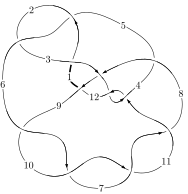
\includegraphics[width=112pt]{../../../GIT/diagram.site/Diagrams/png/2589_12n_0500.png}\\
\ \ \ A knot diagram\footnotemark}&
\allowdisplaybreaks
\textbf{Linearized knot diagam} \\
\cline{2-2}
 &
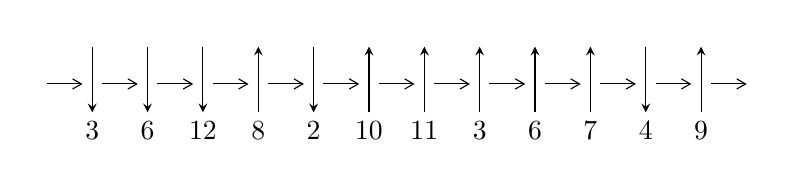
\begin{tikzpicture}[x=20pt, y=17pt]
	% nodes
	\node (C0) at (0, 0) {};
	\node (C1) at (1, 0) {};
	\node (C1U) at (1, +1) {};
	\node (C1D) at (1, -1) {3};

	\node (C2) at (2, 0) {};
	\node (C2U) at (2, +1) {};
	\node (C2D) at (2, -1) {6};

	\node (C3) at (3, 0) {};
	\node (C3U) at (3, +1) {};
	\node (C3D) at (3, -1) {12};

	\node (C4) at (4, 0) {};
	\node (C4U) at (4, +1) {};
	\node (C4D) at (4, -1) {8};

	\node (C5) at (5, 0) {};
	\node (C5U) at (5, +1) {};
	\node (C5D) at (5, -1) {2};

	\node (C6) at (6, 0) {};
	\node (C6U) at (6, +1) {};
	\node (C6D) at (6, -1) {10};

	\node (C7) at (7, 0) {};
	\node (C7U) at (7, +1) {};
	\node (C7D) at (7, -1) {11};

	\node (C8) at (8, 0) {};
	\node (C8U) at (8, +1) {};
	\node (C8D) at (8, -1) {3};

	\node (C9) at (9, 0) {};
	\node (C9U) at (9, +1) {};
	\node (C9D) at (9, -1) {6};

	\node (C10) at (10, 0) {};
	\node (C10U) at (10, +1) {};
	\node (C10D) at (10, -1) {7};

	\node (C11) at (11, 0) {};
	\node (C11U) at (11, +1) {};
	\node (C11D) at (11, -1) {4};

	\node (C12) at (12, 0) {};
	\node (C12U) at (12, +1) {};
	\node (C12D) at (12, -1) {9};
	\node (C13) at (13, 0) {};

	% arrows
	\draw[->,>={angle 60}]
	(C0) edge (C1) (C1) edge (C2) (C2) edge (C3) (C3) edge (C4) (C4) edge (C5) (C5) edge (C6) (C6) edge (C7) (C7) edge (C8) (C8) edge (C9) (C9) edge (C10) (C10) edge (C11) (C11) edge (C12) (C12) edge (C13) ;	\draw[->,>=stealth]
	(C1U) edge (C1D) (C2U) edge (C2D) (C3U) edge (C3D) (C4D) edge (C4U) (C5U) edge (C5D) (C6D) edge (C6U) (C7D) edge (C7U) (C8D) edge (C8U) (C9D) edge (C9U) (C10D) edge (C10U) (C11U) edge (C11D) (C12D) edge (C12U) ;
	\end{tikzpicture} \\
\hhline{~~} \\& 
\textbf{Solving Sequence} \\ \cline{2-2} 
 &
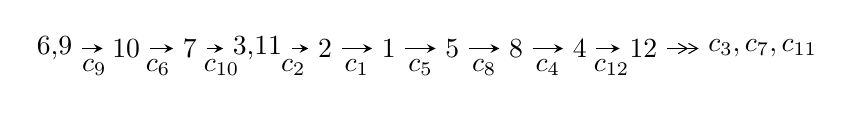
\begin{tikzpicture}[x=23pt, y=7pt]
	% node
	\node (A0) at (-1/8, 0) {6,9};
	\node (A1) at (1, 0) {10};
	\node (A2) at (2, 0) {7};
	\node (A3) at (49/16, 0) {3,11};
	\node (A4) at (33/8, 0) {2};
	\node (A5) at (41/8, 0) {1};
	\node (A6) at (49/8, 0) {5};
	\node (A7) at (57/8, 0) {8};
	\node (A8) at (65/8, 0) {4};
	\node (A9) at (73/8, 0) {12};
	\node (C1) at (1/2, -1) {$c_{9}$};
	\node (C2) at (3/2, -1) {$c_{6}$};
	\node (C3) at (5/2, -1) {$c_{10}$};
	\node (C4) at (29/8, -1) {$c_{2}$};
	\node (C5) at (37/8, -1) {$c_{1}$};
	\node (C6) at (45/8, -1) {$c_{5}$};
	\node (C7) at (53/8, -1) {$c_{8}$};
	\node (C8) at (61/8, -1) {$c_{4}$};
	\node (C9) at (69/8, -1) {$c_{12}$};
	\node (A10) at (11, 0) {$c_{3},c_{7},c_{11}$};

	% edge
	\draw[->,>=stealth]	
	(A0) edge (A1) (A1) edge (A2) (A2) edge (A3) (A3) edge (A4) (A4) edge (A5) (A5) edge (A6) (A6) edge (A7) (A7) edge (A8) (A8) edge (A9) ;
	\draw[->>,>={angle 60}]	
	(A9) edge (A10);
\end{tikzpicture} \\ 

\end{tabular} \\

\footnotetext{
The image of knot diagram is generated by the software ``\textbf{Draw programme}" developed by Andrew Bartholomew(\url{http://www.layer8.co.uk/maths/draw/index.htm\#Running-draw}), where we modified some parts for our purpose(\url{https://github.com/CATsTAILs/LinksPainter}).
}\phantom \\ \newline 
\centering \textbf{Ideals for irreducible components\footnotemark of $X_{\text{par}}$} 
 
\begin{align*}
I^u_{1}&=\langle 
5 u^{30}-14 u^{29}+\cdots+2 b+5,\;- u^{30}+2 u^{29}+\cdots+4 a+5,\;u^{31}-4 u^{30}+\cdots-2 u-1\rangle \\
I^u_{2}&=\langle 
b,\;a^3+a^2 u+a^2-2 u-3,\;u^2+u-1\rangle \\
\\
\end{align*}
\raggedright * 2 irreducible components of $\dim_{\mathbb{C}}=0$, with total 37 representations.\\
\footnotetext{All coefficients of polynomials are rational numbers. But the coefficients are sometimes approximated in decimal forms when there is not enough margin.}
\newpage
\renewcommand{\arraystretch}{1}
\centering \section*{I. $I^u_{1}= \langle 5 u^{30}-14 u^{29}+\cdots+2 b+5,\;- u^{30}+2 u^{29}+\cdots+4 a+5,\;u^{31}-4 u^{30}+\cdots-2 u-1 \rangle$}
\flushleft \textbf{(i) Arc colorings}\\
\begin{tabular}{m{7pt} m{180pt} m{7pt} m{180pt} }
\flushright $a_{6}=$&$\begin{pmatrix}0\\u\end{pmatrix}$ \\
\flushright $a_{9}=$&$\begin{pmatrix}1\\0\end{pmatrix}$ \\
\flushright $a_{10}=$&$\begin{pmatrix}1\\- u^2\end{pmatrix}$ \\
\flushright $a_{7}=$&$\begin{pmatrix}u\\- u^3+u\end{pmatrix}$ \\
\flushright $a_{3}=$&$\begin{pmatrix}\frac{1}{4} u^{30}-\frac{1}{2} u^{29}+\cdots-\frac{5}{2} u-\frac{5}{4}\\-\frac{5}{2} u^{30}+7 u^{29}+\cdots-6 u-\frac{5}{2}\end{pmatrix}$ \\
\flushright $a_{11}=$&$\begin{pmatrix}- u^2+1\\u^4-2 u^2\end{pmatrix}$ \\
\flushright $a_{2}=$&$\begin{pmatrix}\frac{1}{4} u^{30}-\frac{1}{2} u^{29}+\cdots-\frac{5}{2} u-\frac{5}{4}\\-\frac{13}{4} u^{30}+\frac{33}{4} u^{29}+\cdots-\frac{29}{4} u-3\end{pmatrix}$ \\
\flushright $a_{1}=$&$\begin{pmatrix}\frac{9}{4} u^{30}-\frac{15}{4} u^{29}+\cdots+\frac{21}{4} u+\frac{5}{2}\\-\frac{5}{4} u^{30}+\frac{13}{4} u^{29}+\cdots-\frac{9}{4} u-1\end{pmatrix}$ \\
\flushright $a_{5}=$&$\begin{pmatrix}-\frac{1}{4} u^{29}+\frac{3}{4} u^{28}+\cdots-\frac{17}{4} u+\frac{3}{4}\\\frac{1}{4} u^{30}-\frac{1}{2} u^{29}+\cdots+\frac{1}{2} u+\frac{1}{4}\end{pmatrix}$ \\
\flushright $a_{8}=$&$\begin{pmatrix}- u^3+2 u\\u^5-3 u^3+u\end{pmatrix}$ \\
\flushright $a_{4}=$&$\begin{pmatrix}-\frac{1}{4} u^{30}+\frac{1}{4} u^{29}+\cdots-\frac{19}{4} u+\frac{1}{2}\\\frac{1}{4} u^{30}-\frac{1}{2} u^{29}+\cdots+\frac{1}{2} u+\frac{1}{4}\end{pmatrix}$ \\
\flushright $a_{12}=$&$\begin{pmatrix}\frac{7}{2} u^{30}-7 u^{29}+\cdots+\frac{15}{2} u+\frac{7}{2}\\-\frac{5}{4} u^{30}+\frac{13}{4} u^{29}+\cdots-\frac{9}{4} u-1\end{pmatrix}$\\&\end{tabular}
\flushleft \textbf{(ii) Obstruction class $= -1$}\\~\\
\flushleft \textbf{(iii) Cusp Shapes $= -11 u^{30}+29 u^{29}+\cdots-16 u^2-\frac{15}{2}$}\\~\\
\newpage\renewcommand{\arraystretch}{1}
\flushleft \textbf{(iv) u-Polynomials at the component}\newline \\
\begin{tabular}{m{50pt}|m{274pt}}
Crossings & \hspace{64pt}u-Polynomials at each crossing \\
\hline $$\begin{aligned}c_{1}\end{aligned}$$&$\begin{aligned}
&u^{31}+35 u^{30}+\cdots+177 u+4
\end{aligned}$\\
\hline $$\begin{aligned}c_{2},c_{5}\end{aligned}$$&$\begin{aligned}
&u^{31}+3 u^{30}+\cdots-15 u+2
\end{aligned}$\\
\hline $$\begin{aligned}c_{3},c_{11}\end{aligned}$$&$\begin{aligned}
&u^{31}-3 u^{30}+\cdots-9 u+1
\end{aligned}$\\
\hline $$\begin{aligned}c_{4}\end{aligned}$$&$\begin{aligned}
&u^{31}-3 u^{30}+\cdots-2916 u+243
\end{aligned}$\\
\hline $$\begin{aligned}c_{6},c_{7},c_{9}\\c_{10}\end{aligned}$$&$\begin{aligned}
&u^{31}-4 u^{30}+\cdots-2 u-1
\end{aligned}$\\
\hline $$\begin{aligned}c_{8}\end{aligned}$$&$\begin{aligned}
&u^{31}+u^{30}+\cdots-32 u+64
\end{aligned}$\\
\hline $$\begin{aligned}c_{12}\end{aligned}$$&$\begin{aligned}
&u^{31}+22 u^{29}+\cdots-2095 u+2071
\end{aligned}$\\
\hline
\end{tabular}\\~\\
\newpage\renewcommand{\arraystretch}{1}
\flushleft \textbf{(v) Riley Polynomials at the component}\newline \\
\begin{tabular}{m{50pt}|m{274pt}}
Crossings & \hspace{64pt}Riley Polynomials at each crossing \\
\hline $$\begin{aligned}c_{1}\end{aligned}$$&$\begin{aligned}
&y^{31}-75 y^{30}+\cdots+52609 y-16
\end{aligned}$\\
\hline $$\begin{aligned}c_{2},c_{5}\end{aligned}$$&$\begin{aligned}
&y^{31}-35 y^{30}+\cdots+177 y-4
\end{aligned}$\\
\hline $$\begin{aligned}c_{3},c_{11}\end{aligned}$$&$\begin{aligned}
&y^{31}+25 y^{30}+\cdots+65 y-1
\end{aligned}$\\
\hline $$\begin{aligned}c_{4}\end{aligned}$$&$\begin{aligned}
&y^{31}+5 y^{30}+\cdots+3359232 y-59049
\end{aligned}$\\
\hline $$\begin{aligned}c_{6},c_{7},c_{9}\\c_{10}\end{aligned}$$&$\begin{aligned}
&y^{31}-34 y^{30}+\cdots-2 y-1
\end{aligned}$\\
\hline $$\begin{aligned}c_{8}\end{aligned}$$&$\begin{aligned}
&y^{31}+35 y^{30}+\cdots+1024 y-4096
\end{aligned}$\\
\hline $$\begin{aligned}c_{12}\end{aligned}$$&$\begin{aligned}
&y^{31}+44 y^{30}+\cdots-9225729 y-4289041
\end{aligned}$\\
\hline
\end{tabular}\\~\\
\newpage\flushleft \textbf{(vi) Complex Volumes and Cusp Shapes}
$$\begin{array}{c|c|c}  
\text{Solutions to }I^u_{1}& \I (\text{vol} + \sqrt{-1}CS) & \text{Cusp shape}\\
 \hline 
\begin{aligned}
u &= -0.602350 + 0.764489 I \\
a &= -0.96517 - 1.53953 I \\
b &= \phantom{-}0.35606 - 1.75288 I\end{aligned}
 & -5.83199 - 7.50635 I & \phantom{-}2.66894 + 5.59456 I \\ \hline\begin{aligned}
u &= -0.602350 - 0.764489 I \\
a &= -0.96517 + 1.53953 I \\
b &= \phantom{-}0.35606 + 1.75288 I\end{aligned}
 & -5.83199 + 7.50635 I & \phantom{-}2.66894 - 5.59456 I \\ \hline\begin{aligned}
u &= -0.543360 + 0.792514 I \\
a &= \phantom{-}0.91165 + 1.54215 I \\
b &= -0.17449 + 1.80984 I\end{aligned}
 & -10.03040 - 2.62343 I & -1.03684 + 2.68072 I \\ \hline\begin{aligned}
u &= -0.543360 - 0.792514 I \\
a &= \phantom{-}0.91165 - 1.54215 I \\
b &= -0.17449 - 1.80984 I\end{aligned}
 & -10.03040 + 2.62343 I & -1.03684 - 2.68072 I \\ \hline\begin{aligned}
u &= -0.473452 + 0.802011 I \\
a &= -0.85502 - 1.55001 I \\
b &= -0.03027 - 1.79370 I\end{aligned}
 & -6.21873 + 2.31735 I & \phantom{-}1.87364 - 0.58111 I \\ \hline\begin{aligned}
u &= -0.473452 - 0.802011 I \\
a &= -0.85502 + 1.55001 I \\
b &= -0.03027 + 1.79370 I\end{aligned}
 & -6.21873 - 2.31735 I & \phantom{-}1.87364 + 0.58111 I \\ \hline\begin{aligned}
u &= \phantom{-}0.751448 + 0.311977 I \\
a &= -0.131566 - 0.324454 I \\
b &= -0.652866 + 0.653689 I\end{aligned}
 & \phantom{-}3.50508 + 0.49905 I & \phantom{-}6.93091 - 1.38994 I \\ \hline\begin{aligned}
u &= \phantom{-}0.751448 - 0.311977 I \\
a &= -0.131566 + 0.324454 I \\
b &= -0.652866 - 0.653689 I\end{aligned}
 & \phantom{-}3.50508 - 0.49905 I & \phantom{-}6.93091 + 1.38994 I \\ \hline\begin{aligned}
u &= -1.34946\phantom{ +0.000000I} \\
a &= -0.997928\phantom{ +0.000000I} \\
b &= \phantom{-}1.24408\phantom{ +0.000000I}\end{aligned}
 & \phantom{-}2.46733\phantom{ +0.000000I} & \phantom{-}3.43490\phantom{ +0.000000I} \\ \hline\begin{aligned}
u &= \phantom{-}1.366810 + 0.074394 I \\
a &= \phantom{-}0.234215 - 0.622051 I \\
b &= -0.045603 - 1.264260 I\end{aligned}
 & \phantom{-}3.50947 + 1.97376 I & \phantom{-}4.13605 - 3.59471 I\\
 \hline 
 \end{array}$$\newpage$$\begin{array}{c|c|c}  
\text{Solutions to }I^u_{1}& \I (\text{vol} + \sqrt{-1}CS) & \text{Cusp shape}\\
 \hline 
\begin{aligned}
u &= \phantom{-}1.366810 - 0.074394 I \\
a &= \phantom{-}0.234215 + 0.622051 I \\
b &= -0.045603 + 1.264260 I\end{aligned}
 & \phantom{-}3.50947 - 1.97376 I & \phantom{-}4.13605 + 3.59471 I \\ \hline\begin{aligned}
u &= -1.375110 + 0.092603 I \\
a &= \phantom{-}0.939498 + 0.219836 I \\
b &= -1.276320 - 0.062520 I\end{aligned}
 & \phantom{-}6.34649 - 4.23203 I & \phantom{-}7.34906 + 3.43500 I \\ \hline\begin{aligned}
u &= -1.375110 - 0.092603 I \\
a &= \phantom{-}0.939498 - 0.219836 I \\
b &= -1.276320 + 0.062520 I\end{aligned}
 & \phantom{-}6.34649 + 4.23203 I & \phantom{-}7.34906 - 3.43500 I \\ \hline\begin{aligned}
u &= \phantom{-}0.527133\phantom{ +0.000000I} \\
a &= -0.257315\phantom{ +0.000000I} \\
b &= \phantom{-}0.358345\phantom{ +0.000000I}\end{aligned}
 & \phantom{-}0.784642\phantom{ +0.000000I} & \phantom{-}13.1720\phantom{ +0.000000I} \\ \hline\begin{aligned}
u &= \phantom{-}1.47433 + 0.08812 I \\
a &= -0.497026 + 0.970443 I \\
b &= \phantom{-}0.186128 + 1.163550 I\end{aligned}
 & \phantom{-}9.65588 + 4.45983 I & \phantom{-}7.97346 - 3.71466 I \\ \hline\begin{aligned}
u &= \phantom{-}1.47433 - 0.08812 I \\
a &= -0.497026 - 0.970443 I \\
b &= \phantom{-}0.186128 - 1.163550 I\end{aligned}
 & \phantom{-}9.65588 - 4.45983 I & \phantom{-}7.97346 + 3.71466 I \\ \hline\begin{aligned}
u &= \phantom{-}0.146677 + 0.492597 I \\
a &= -0.018556 + 1.292810 I \\
b &= \phantom{-}0.836447 + 0.454443 I\end{aligned}
 & \phantom{-}1.62298 + 2.35384 I & \phantom{-}1.82470 - 4.53214 I \\ \hline\begin{aligned}
u &= \phantom{-}0.146677 - 0.492597 I \\
a &= -0.018556 - 1.292810 I \\
b &= \phantom{-}0.836447 - 0.454443 I\end{aligned}
 & \phantom{-}1.62298 - 2.35384 I & \phantom{-}1.82470 + 4.53214 I \\ \hline\begin{aligned}
u &= \phantom{-}1.49116 + 0.29858 I \\
a &= \phantom{-}0.877997 - 0.367679 I \\
b &= -0.35046 - 1.70481 I\end{aligned}
 & \phantom{-}0.10746 + 1.69492 I & \phantom{-0.000000 } 0 \\ \hline\begin{aligned}
u &= \phantom{-}1.49116 - 0.29858 I \\
a &= \phantom{-}0.877997 + 0.367679 I \\
b &= -0.35046 + 1.70481 I\end{aligned}
 & \phantom{-}0.10746 - 1.69492 I & \phantom{-0.000000 } 0\\
 \hline 
 \end{array}$$\newpage$$\begin{array}{c|c|c}  
\text{Solutions to }I^u_{1}& \I (\text{vol} + \sqrt{-1}CS) & \text{Cusp shape}\\
 \hline 
\begin{aligned}
u &= \phantom{-}1.54074 + 0.28653 I \\
a &= -0.983728 + 0.406676 I \\
b &= \phantom{-}0.52058 + 1.68308 I\end{aligned}
 & -3.24464 + 6.59865 I & \phantom{-0.000000 } 0 \\ \hline\begin{aligned}
u &= \phantom{-}1.54074 - 0.28653 I \\
a &= -0.983728 - 0.406676 I \\
b &= \phantom{-}0.52058 - 1.68308 I\end{aligned}
 & -3.24464 - 6.59865 I & \phantom{-0.000000 } 0 \\ \hline\begin{aligned}
u &= -0.369500 + 0.215346 I \\
a &= \phantom{-}0.63729 + 2.88917 I \\
b &= -0.010339 + 0.599954 I\end{aligned}
 & \phantom{-}3.53058 - 3.26263 I & -0.32878 + 7.06957 I \\ \hline\begin{aligned}
u &= -0.369500 - 0.215346 I \\
a &= \phantom{-}0.63729 - 2.88917 I \\
b &= -0.010339 - 0.599954 I\end{aligned}
 & \phantom{-}3.53058 + 3.26263 I & -0.32878 - 7.06957 I \\ \hline\begin{aligned}
u &= \phantom{-}1.57119 + 0.26571 I \\
a &= \phantom{-}1.058660 - 0.452456 I \\
b &= -0.63708 - 1.61140 I\end{aligned}
 & \phantom{-}1.31297 + 11.33500 I & \phantom{-0.000000 } 0 \\ \hline\begin{aligned}
u &= \phantom{-}1.57119 - 0.26571 I \\
a &= \phantom{-}1.058660 + 0.452456 I \\
b &= -0.63708 + 1.61140 I\end{aligned}
 & \phantom{-}1.31297 - 11.33500 I & \phantom{-0.000000 } 0 \\ \hline\begin{aligned}
u &= -1.59573\phantom{ +0.000000I} \\
a &= \phantom{-}0.257600\phantom{ +0.000000I} \\
b &= -0.497580\phantom{ +0.000000I}\end{aligned}
 & \phantom{-}8.24985\phantom{ +0.000000I} & \phantom{-}15.5880\phantom{ +0.000000I} \\ \hline\begin{aligned}
u &= -1.63289 + 0.05265 I \\
a &= -0.234203 - 0.321554 I \\
b &= \phantom{-}0.531375 + 0.618506 I\end{aligned}
 & \phantom{-}11.78470 - 1.72102 I & \phantom{-0.000000 } 0 \\ \hline\begin{aligned}
u &= -1.63289 - 0.05265 I \\
a &= -0.234203 + 0.321554 I \\
b &= \phantom{-}0.531375 - 0.618506 I\end{aligned}
 & \phantom{-}11.78470 + 1.72102 I & \phantom{-0.000000 } 0 \\ \hline\begin{aligned}
u &= -0.136671 + 0.320613 I \\
a &= \phantom{-}0.02478 - 2.19557 I \\
b &= -0.305592 - 0.594543 I\end{aligned}
 & -1.239080 - 0.576153 I & -5.00436 + 2.78236 I\\
 \hline 
 \end{array}$$\newpage$$\begin{array}{c|c|c}  
\text{Solutions to }I^u_{1}& \I (\text{vol} + \sqrt{-1}CS) & \text{Cusp shape}\\
 \hline 
\begin{aligned}
u &= -0.136671 - 0.320613 I \\
a &= \phantom{-}0.02478 + 2.19557 I \\
b &= -0.305592 + 0.594543 I\end{aligned}
 & -1.239080 + 0.576153 I & -5.00436 - 2.78236 I\\
 \hline 
 \end{array}$$\newpage\newpage\renewcommand{\arraystretch}{1}
\centering \section*{II. $I^u_{2}= \langle b,\;a^3+a^2 u+a^2-2 u-3,\;u^2+u-1 \rangle$}
\flushleft \textbf{(i) Arc colorings}\\
\begin{tabular}{m{7pt} m{180pt} m{7pt} m{180pt} }
\flushright $a_{6}=$&$\begin{pmatrix}0\\u\end{pmatrix}$ \\
\flushright $a_{9}=$&$\begin{pmatrix}1\\0\end{pmatrix}$ \\
\flushright $a_{10}=$&$\begin{pmatrix}1\\u-1\end{pmatrix}$ \\
\flushright $a_{7}=$&$\begin{pmatrix}u\\- u+1\end{pmatrix}$ \\
\flushright $a_{3}=$&$\begin{pmatrix}a\\0\end{pmatrix}$ \\
\flushright $a_{11}=$&$\begin{pmatrix}u\\- u\end{pmatrix}$ \\
\flushright $a_{2}=$&$\begin{pmatrix}a\\a u- a\end{pmatrix}$ \\
\flushright $a_{1}=$&$\begin{pmatrix}a^2 u+a- u-1\\a u- a\end{pmatrix}$ \\
\flushright $a_{5}=$&$\begin{pmatrix}a^2 u\\-2 a^2 u+a^2+u\end{pmatrix}$ \\
\flushright $a_{8}=$&$\begin{pmatrix}1\\0\end{pmatrix}$ \\
\flushright $a_{4}=$&$\begin{pmatrix}3 a^2 u- a^2- u\\-2 a^2 u+a^2+u\end{pmatrix}$ \\
\flushright $a_{12}=$&$\begin{pmatrix}a^2 u- a u+2 a- u-1\\a u- a\end{pmatrix}$\\&\end{tabular}
\flushleft \textbf{(ii) Obstruction class $= 1$}\\~\\
\flushleft \textbf{(iii) Cusp Shapes $= - a^2-6 a u+a+u+5$}\\~\\
\newpage\renewcommand{\arraystretch}{1}
\flushleft \textbf{(iv) u-Polynomials at the component}\newline \\
\begin{tabular}{m{50pt}|m{274pt}}
Crossings & \hspace{64pt}u-Polynomials at each crossing \\
\hline $$\begin{aligned}c_{1},c_{11}\end{aligned}$$&$\begin{aligned}
&(u^3- u^2+2 u-1)^2
\end{aligned}$\\
\hline $$\begin{aligned}c_{2}\end{aligned}$$&$\begin{aligned}
&(u^3+u^2-1)^2
\end{aligned}$\\
\hline $$\begin{aligned}c_{3}\end{aligned}$$&$\begin{aligned}
&(u^3+u^2+2 u+1)^2
\end{aligned}$\\
\hline $$\begin{aligned}c_{4}\end{aligned}$$&$\begin{aligned}
&u^6-2 u^5+5 u^4+2 u^3+3 u^2-3 u-1
\end{aligned}$\\
\hline $$\begin{aligned}c_{5}\end{aligned}$$&$\begin{aligned}
&(u^3- u^2+1)^2
\end{aligned}$\\
\hline $$\begin{aligned}c_{6},c_{7}\end{aligned}$$&$\begin{aligned}
&(u^2- u-1)^3
\end{aligned}$\\
\hline $$\begin{aligned}c_{8}\end{aligned}$$&$\begin{aligned}
&u^6
\end{aligned}$\\
\hline $$\begin{aligned}c_{9},c_{10}\end{aligned}$$&$\begin{aligned}
&(u^2+u-1)^3
\end{aligned}$\\
\hline $$\begin{aligned}c_{12}\end{aligned}$$&$\begin{aligned}
&u^6- u^5- u^4+4 u^3+3 u^2-1
\end{aligned}$\\
\hline
\end{tabular}\\~\\
\newpage\renewcommand{\arraystretch}{1}
\flushleft \textbf{(v) Riley Polynomials at the component}\newline \\
\begin{tabular}{m{50pt}|m{274pt}}
Crossings & \hspace{64pt}Riley Polynomials at each crossing \\
\hline $$\begin{aligned}c_{1},c_{3},c_{11}\end{aligned}$$&$\begin{aligned}
&(y^3+3 y^2+2 y-1)^2
\end{aligned}$\\
\hline $$\begin{aligned}c_{2},c_{5}\end{aligned}$$&$\begin{aligned}
&(y^3- y^2+2 y-1)^2
\end{aligned}$\\
\hline $$\begin{aligned}c_{4}\end{aligned}$$&$\begin{aligned}
&y^6+6 y^5+39 y^4+12 y^3+11 y^2-15 y+1
\end{aligned}$\\
\hline $$\begin{aligned}c_{6},c_{7},c_{9}\\c_{10}\end{aligned}$$&$\begin{aligned}
&(y^2-3 y+1)^3
\end{aligned}$\\
\hline $$\begin{aligned}c_{8}\end{aligned}$$&$\begin{aligned}
&y^6
\end{aligned}$\\
\hline $$\begin{aligned}c_{12}\end{aligned}$$&$\begin{aligned}
&y^6-3 y^5+15 y^4-24 y^3+11 y^2-6 y+1
\end{aligned}$\\
\hline
\end{tabular}\\~\\
\newpage\flushleft \textbf{(vi) Complex Volumes and Cusp Shapes}
$$\begin{array}{c|c|c}  
\text{Solutions to }I^u_{2}& \I (\text{vol} + \sqrt{-1}CS) & \text{Cusp shape}\\
 \hline 
\begin{aligned}
u &= \phantom{-}0.618034\phantom{ +0.000000I} \\
a &= \phantom{-}1.22142\phantom{ +0.000000I} \\
b &= \phantom{-0.000000 } 0\end{aligned}
 & -0.126494\phantom{ +0.000000I} & \phantom{-}0.818320\phantom{ +0.000000I} \\ \hline\begin{aligned}
u &= \phantom{-}0.618034\phantom{ +0.000000I} \\
a &= -1.41973 + 1.20521 I \\
b &= \phantom{-0.000000 } 0\end{aligned}
 & \phantom{-}4.01109 + 2.82812 I & \phantom{-}8.89985 + 0.15818 I \\ \hline\begin{aligned}
u &= \phantom{-}0.618034\phantom{ +0.000000I} \\
a &= -1.41973 - 1.20521 I \\
b &= \phantom{-0.000000 } 0\end{aligned}
 & \phantom{-}4.01109 - 2.82812 I & \phantom{-}8.89985 - 0.15818 I \\ \hline\begin{aligned}
u &= -1.61803\phantom{ +0.000000I} \\
a &= \phantom{-}0.542287 + 0.460350 I \\
b &= \phantom{-0.000000 } 0\end{aligned}
 & \phantom{-}11.90680 - 2.82812 I & \phantom{-}9.10673 + 4.43024 I \\ \hline\begin{aligned}
u &= -1.61803\phantom{ +0.000000I} \\
a &= \phantom{-}0.542287 - 0.460350 I \\
b &= \phantom{-0.000000 } 0\end{aligned}
 & \phantom{-}11.90680 + 2.82812 I & \phantom{-}9.10673 - 4.43024 I \\ \hline\begin{aligned}
u &= -1.61803\phantom{ +0.000000I} \\
a &= -0.466540\phantom{ +0.000000I} \\
b &= \phantom{-0.000000 } 0\end{aligned}
 & \phantom{-}7.76919\phantom{ +0.000000I} & -1.83150\phantom{ +0.000000I}\\
 \hline 
 \end{array}$$\newpage
\newpage\renewcommand{\arraystretch}{1}
\centering \section*{ III. u-Polynomials}
\begin{tabular}{m{50pt}|m{274pt}}
Crossings & \hspace{64pt}u-Polynomials at each crossing \\
\hline $$\begin{aligned}c_{1}\end{aligned}$$&$\begin{aligned}
&((u^3- u^2+2 u-1)^2)(u^{31}+35 u^{30}+\cdots+177 u+4)
\end{aligned}$\\
\hline $$\begin{aligned}c_{2}\end{aligned}$$&$\begin{aligned}
&((u^3+u^2-1)^2)(u^{31}+3 u^{30}+\cdots-15 u+2)
\end{aligned}$\\
\hline $$\begin{aligned}c_{3}\end{aligned}$$&$\begin{aligned}
&((u^3+u^2+2 u+1)^2)(u^{31}-3 u^{30}+\cdots-9 u+1)
\end{aligned}$\\
\hline $$\begin{aligned}c_{4}\end{aligned}$$&$\begin{aligned}
&(u^6-2 u^5+\cdots-3 u-1)(u^{31}-3 u^{30}+\cdots-2916 u+243)
\end{aligned}$\\
\hline $$\begin{aligned}c_{5}\end{aligned}$$&$\begin{aligned}
&((u^3- u^2+1)^2)(u^{31}+3 u^{30}+\cdots-15 u+2)
\end{aligned}$\\
\hline $$\begin{aligned}c_{6},c_{7}\end{aligned}$$&$\begin{aligned}
&((u^2- u-1)^3)(u^{31}-4 u^{30}+\cdots-2 u-1)
\end{aligned}$\\
\hline $$\begin{aligned}c_{8}\end{aligned}$$&$\begin{aligned}
&u^6(u^{31}+u^{30}+\cdots-32 u+64)
\end{aligned}$\\
\hline $$\begin{aligned}c_{9},c_{10}\end{aligned}$$&$\begin{aligned}
&((u^2+u-1)^3)(u^{31}-4 u^{30}+\cdots-2 u-1)
\end{aligned}$\\
\hline $$\begin{aligned}c_{11}\end{aligned}$$&$\begin{aligned}
&((u^3- u^2+2 u-1)^2)(u^{31}-3 u^{30}+\cdots-9 u+1)
\end{aligned}$\\
\hline $$\begin{aligned}c_{12}\end{aligned}$$&$\begin{aligned}
&(u^6- u^5- u^4+4 u^3+3 u^2-1)(u^{31}+22 u^{29}+\cdots-2095 u+2071)
\end{aligned}$\\
\hline
\end{tabular}\newpage\renewcommand{\arraystretch}{1}
\centering \section*{ IV. Riley Polynomials}
\begin{tabular}{m{50pt}|m{274pt}}
Crossings & \hspace{64pt}Riley Polynomials at each crossing \\
\hline $$\begin{aligned}c_{1}\end{aligned}$$&$\begin{aligned}
&((y^3+3 y^2+2 y-1)^2)(y^{31}-75 y^{30}+\cdots+52609 y-16)
\end{aligned}$\\
\hline $$\begin{aligned}c_{2},c_{5}\end{aligned}$$&$\begin{aligned}
&((y^3- y^2+2 y-1)^2)(y^{31}-35 y^{30}+\cdots+177 y-4)
\end{aligned}$\\
\hline $$\begin{aligned}c_{3},c_{11}\end{aligned}$$&$\begin{aligned}
&((y^3+3 y^2+2 y-1)^2)(y^{31}+25 y^{30}+\cdots+65 y-1)
\end{aligned}$\\
\hline $$\begin{aligned}c_{4}\end{aligned}$$&$\begin{aligned}
&(y^6+6 y^5+39 y^4+12 y^3+11 y^2-15 y+1)\\
&\cdot(y^{31}+5 y^{30}+\cdots+3359232 y-59049)
\end{aligned}$\\
\hline $$\begin{aligned}c_{6},c_{7},c_{9}\\c_{10}\end{aligned}$$&$\begin{aligned}
&((y^2-3 y+1)^3)(y^{31}-34 y^{30}+\cdots-2 y-1)
\end{aligned}$\\
\hline $$\begin{aligned}c_{8}\end{aligned}$$&$\begin{aligned}
&y^6(y^{31}+35 y^{30}+\cdots+1024 y-4096)
\end{aligned}$\\
\hline $$\begin{aligned}c_{12}\end{aligned}$$&$\begin{aligned}
&(y^6-3 y^5+15 y^4-24 y^3+11 y^2-6 y+1)\\
&\cdot(y^{31}+44 y^{30}+\cdots-9225729 y-4289041)
\end{aligned}$\\
\hline
\end{tabular}
\vskip 2pc
\end{document}